\documentclass[11pt]{beamer}
\usepackage[utf8]{inputenc}
\usepackage[T1]{fontenc}
\usepackage{lmodern}
\usetheme{default}
	\usefonttheme[onlymath]{serif}

\usepackage{graphicx}
	\graphicspath{{Pictures/}}
\usepackage{subfig}
\captionsetup[subfloat]{labelformat=empty}
\captionsetup[figure]{labelformat=empty}

\usepackage{booktabs} % per le tabelle, permette di usare \toprule ecc
\usepackage{amsmath}
\usepackage{mathtools}
\usepackage{multimedia}
\usepackage{hyperref}
\usepackage{ifxetex}
\ifxetex
	\usepackage{fontspec}
	\setsansfont[Scale=0.95]{Arial}
\fi

\begin{document}
	\author{Alessio Raimondi}
	\title{Literature review on non-spherical particles}
	%\subtitle{}
	%\logo{}
	%\institute{}
	%\date{}
	%\subject{}
	%\setbeamercovered{transparent}
	%\setbeamertemplate{navigation symbols}{}
	\begin{frame}[plain]
		\maketitle
	\end{frame}
	
	\begin{frame}
		\centering
		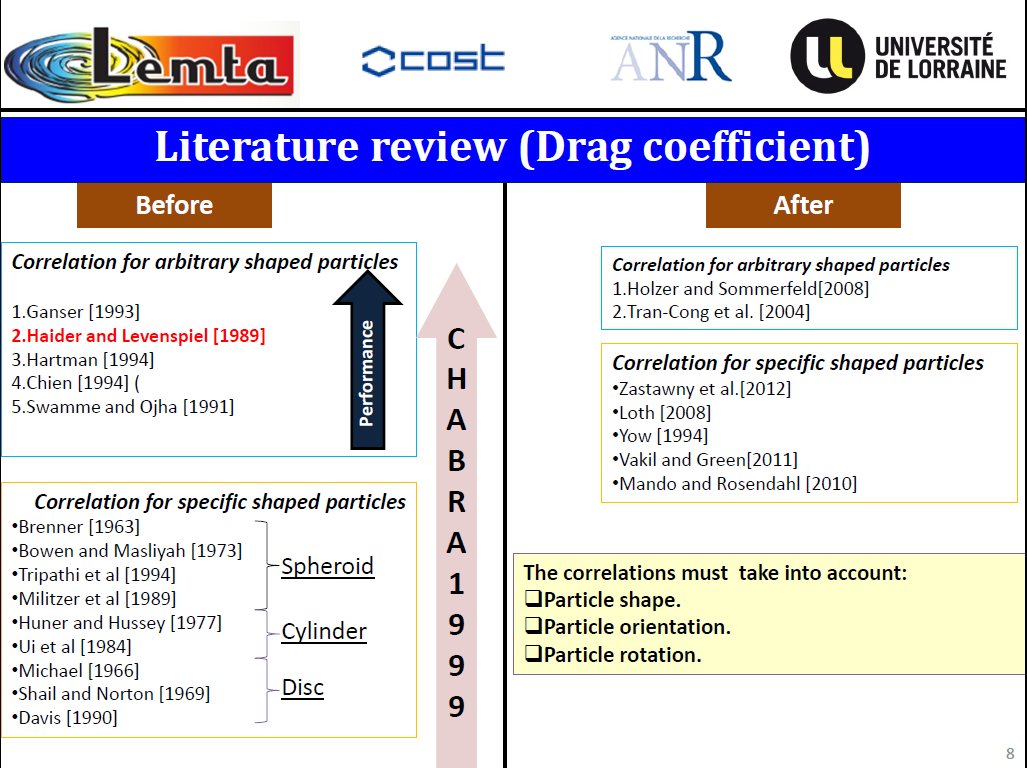
\includegraphics[height=\textheight,width=\textwidth,keepaspectratio]{LiteratureReview.png}		
	\end{frame}

	\begin{frame}{Holzer and Sommerfeld - 2008}
		\begin{itemize}
			\item Huge literature and data review (2061 values)
			\item Interpolation of different previous models
			\item Arbitrary shape (and Orientation!)
			\item Valid for all the Subcritical Regime
		\end{itemize}
	
		\begin{equation*}
			c_D = \frac{8}{Re} \frac{1}{\sqrt{\Phi_{/\!/}}} + \frac{16}{Re} \frac{1}{\Phi} + \frac{3}{\sqrt{Re}} \frac{1}{\Phi^{\frac{3}{4}}} + 0.4210^{0.4(-\log \Phi)^{0.2}} \frac{1}{\Phi_{\perp}}
		\end{equation*}
	\end{frame}

	\begin{frame}{Holzer and Sommerfeld - 2008}
		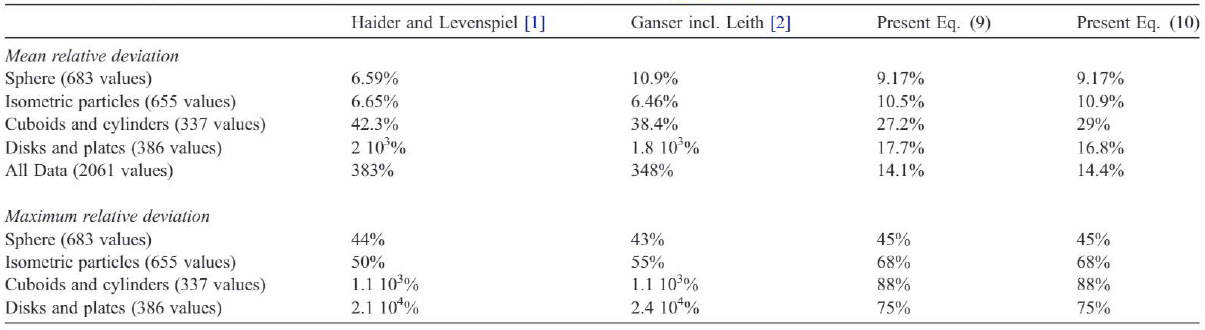
\includegraphics[width=\linewidth]{ComparisonH&S.png}
		\begin{itemize}
			\item Works better than the other for disks and plates
			\item Ganser works better for isometric particles
			\item Works well overall
		\end{itemize}
	\end{frame}

	\begin{frame}{Sanjeevi, Padding and Kuipers -- 2015}
		DNS of a prolate Ellipsoid with $ \Phi = 0.886 $
		\centering
		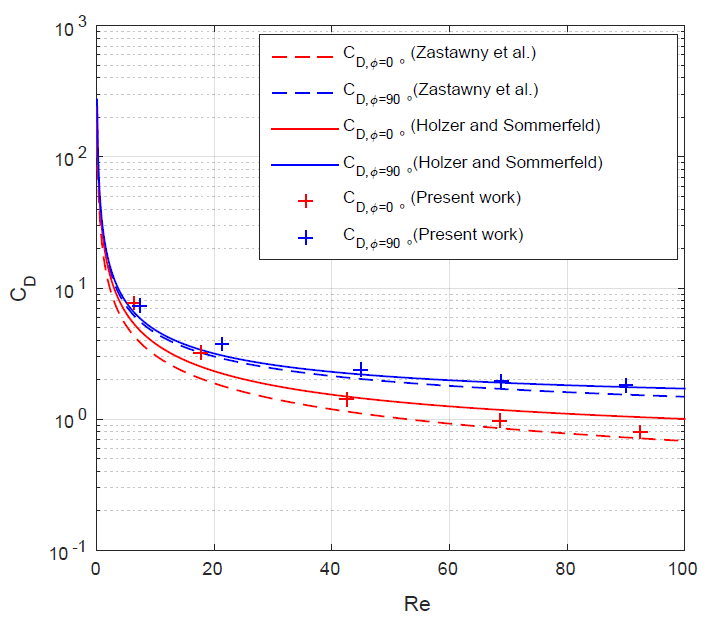
\includegraphics[height=.8\textheight]{DNS.png}
	\end{frame}

	\begin{frame}{Stokes Regime}
		\begin{equation*}
			c_D = \frac{8}{Re} \frac{1}{\sqrt{\Phi_{\perp}}} + \frac{16}{Re} \frac{1}{\Phi}
		\end{equation*}
		\vfill
		\begin{itemize}
			\item Leith's (or Ganser's) model -- 1993
			\item Valid for low Re ($\leq 10$)
			\item For sphere ($ \Phi_{\perp} = \Phi_{/\!/} = \Phi $) degenerates to Stokes' analytical solution
			\item Modification: $ \Phi_{\perp} \rightarrow \Phi_{/\!/} $   (for better approximation of the $ c_D $ as a function of the particle orientation)
		\end{itemize}
	\end{frame}

	\begin{frame}{Newton Regime}
		\begin{block}{Blasius - 1908}
			Friction drag for plates and disks (small cross-sectional area)
			\begin{equation*}
				c_D = 1.327 \cdot 2 \left(\frac{8}{9}\right)^{\frac{1}{4}} \pi^{\frac{1}{4}} \left(\frac{\text{depth}}{\text{length}}\right)^{\frac{1}{4}} \frac{1}{\Phi^{\frac{3}{4}}} \frac{1}{\sqrt{Re}}
			\end{equation*}
			for square plates: \quad $ c_D = 3.43 / (\Phi^{\frac{3}{4}} \sqrt{Re}) $
		\end{block}
	
		\begin{block}{Tran-Cong (2004) and Ganser (1993)}
			Term for high Re proportional to the projected cross-sectional area (Tran-Cong) with the same factor of proportionality of Ganser.
			\begin{equation*}
				c_D = 0.4210^{0.4(-\log \Phi)^{0.2}} \frac{1}{\Phi_{\perp}}
			\end{equation*}
		\end{block}
	\end{frame}

	\begin{frame}{Symbols}
		\begin{block}{Sphericity}
			\begin{columns}[T]
				\begin{column}{.4\textwidth}
					\begin{equation*}
						\Phi = \dfrac{A_{\textup{eq sphere}}}{A_{\textup{particle}}}
					\end{equation*}
				\end{column}
			
				\begin{column}{.6\textwidth}
					Ratio between the surface area of the volume-equivalent sphere and the area of the actual particle
				\end{column}
			\end{columns}
		\end{block}
		\vfill
		\begin{block}{Crosswise Sphericity}
			\begin{columns}[T]
				\begin{column}{.4\textwidth}
					\begin{equation*}
					\Phi_{\perp} = \dfrac{A_{\textup{eq sphere, cross}}} {A_{\textup{particle}, \perp}}
					\end{equation*}
				\end{column}
				
				\begin{column}{.6\textwidth}
					Ratio between the cross-sectional area of the volume-equivalent sphere and the projected cross-sectional area of the actual particle
				\end{column}
			\end{columns}
		\end{block}
	\end{frame}


	\begin{frame}{Symbols}
		\begin{block}{Lengthwise Sphericity}
			\begin{columns}[T]
				\begin{column}{.4\textwidth}
					\begin{equation*}
					\Phi_{/\!/} = \dfrac{A_{\textup{eq sphere, cross}}} {\Delta A}
					\end{equation*}	
					\vfill		
					\begin{equation*}
					\Delta A = \dfrac{A_{\textup{particle}}}{2} - \bar{L_{/\!/}}
					\end{equation*}
				\end{column}
				
				\begin{column}{.6\textwidth}
					Ratio between the cross-sectional area of the volume-equivalent sphere and the difference between half the surface area and the \textit{average} mean longitudinal projected cross-sectional area of the actual particle.\\
					Since $ L_{/\!/} $ depends on the angle of view, an arithmetic average over an entire revolution is used
				\end{column}
			\end{columns}
		\end{block}
	\end{frame}

	\begin{frame}{Recent work -- camera-based methods}
		\begin{block}{China - 2017}
			\centering
			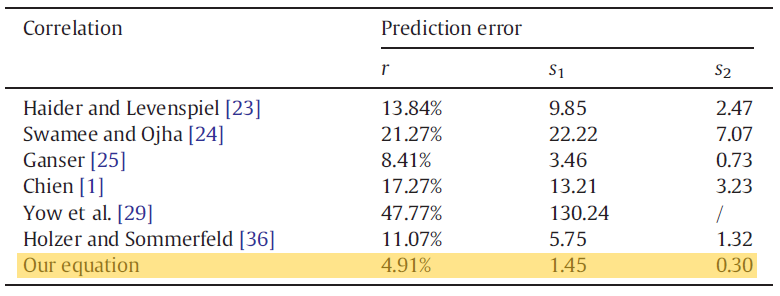
\includegraphics[width=\linewidth]{ComparisonChina.png}\\
			\flushleft
			Limitations: 
			\begin{itemize}
				\item Only three major regular particle shapes investigated (sphere, cube, cylinder)
			\end{itemize}
		\end{block}
	\end{frame}

	\begin{frame}{Recent work -- camera-based methods}
		\begin{block}{Italy (Bari) - 2015}
			\centering
			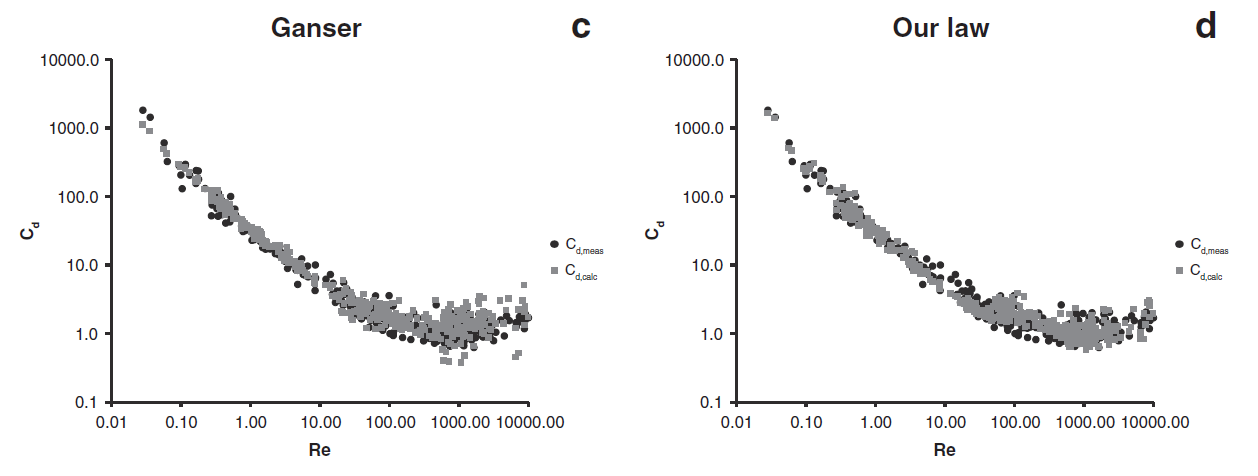
\includegraphics[width=\linewidth]{ComparisonItaly.png}\\
			\flushleft
			Limitations:
			\begin{itemize}
				\item Small data sample
				\item No comparison with Holzer and Sommerfeld (although good agreement with Ganser)
			\end{itemize} 
		\end{block}
	\end{frame}

	\begin{frame}{To do list}
		\begin{itemize}
			\item Read Loth-2008 (Snow??)
			\item Replicate the work of the workshop on SU2
			\item (Try the H\&S formula on the Italian data)
		\end{itemize}
	\end{frame}
\end{document}